\subsubsection{Eliminar Empleado}
En la siguiente imagen \ref{fig:Diagrama de Secuencia - Eliminar Empleado}, se muestra el diagrama de secuencia correspondiente a la eliminación de algún registro de un empleado, esto en el caso de que ya no pertenezca a la organización o simplemente renunció. El sistema muestra un 'mensaje de seguridad' para verificar al administrador si esta seguro de borrar ese registro de la base de datos. Existen dos posibilidades dentro de este módulo:
\begin{itemize}
	\item \textbf{Aceptación:} El administrador acepta que desea eliminar ese registro, el sistema solicita a la base de datos la eliminación de dicho registro y se muestra un mensaje de que el empleado ha sido eliminado de manera satisfactoria.
	\item \textbf{Cancelación:} Si elige la opción 'Cancelar' en la interfaz de usuario, el sistema desaparece el 'mensaje de seguridad' y la base de datos queda intacta. 
\end{itemize}
\begin{figure}[!h]
	\centering
	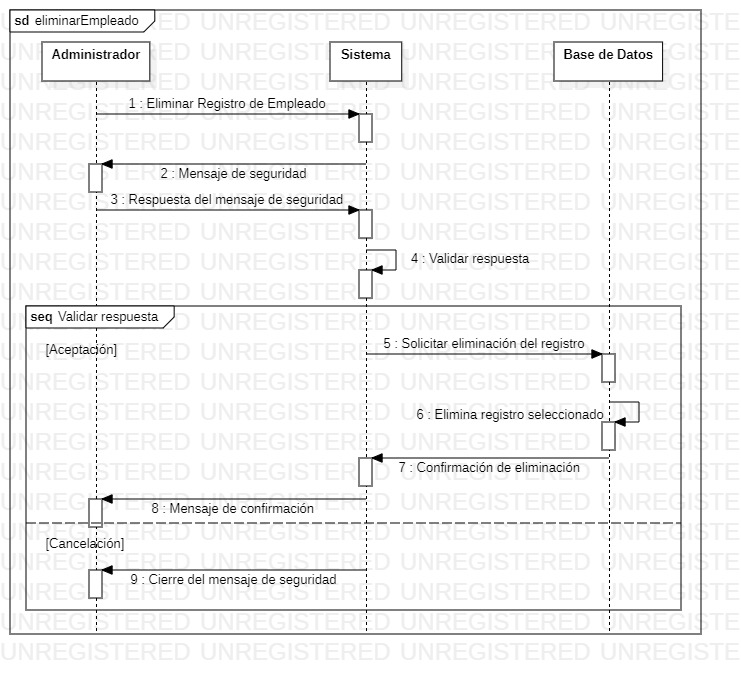
\includegraphics[width=0.8\textwidth]{./diseno/vprocesos/imagenes/eliminarEmpleado}
	\caption{Diagrama de Secuencia - Eliminar Empleado}
	\label{fig:Diagrama de Secuencia - Eliminar Empleado}
\end{figure}
\clearpage